% Options for packages loaded elsewhere
\PassOptionsToPackage{unicode}{hyperref}
\PassOptionsToPackage{hyphens}{url}
\documentclass[12pt, ]{article}

\usepackage{mathtools}
\usepackage{amsmath}
\usepackage{amsthm}
\usepackage{amssymb}
\usepackage[italicdiff]{physics}
\mathtoolsset{showonlyrefs}

% SPACING AND FONTS %%%%%%%%%%%%%%%%%%%%%%%%%%%%%%%%%%%%%%%%%%%%%%%%%%%%%%%%%%%%
\usepackage{iftex}
% CAREFUL: the order of font includes here is very important!
\ifPDFTeX
  \usepackage[OT1,T1]{fontenc}
  \usepackage[utf8]{inputenc}
  \usepackage{textcomp} % provide euro and other symbols
    \usepackage[p,osf,swashQ]{cochineal}
  \usepackage[cochineal,vvarbb]{newtxmath}
      \usepackage[scale=0.95]{biolinum}
    \usepackage[scale=0.95,varl]{inconsolata}
\else % if luatex or xetex
  \usepackage[scale=0.95,varl]{inconsolata}
  \usepackage{newpxtext}
  \usepackage{mathpazo}
    \usepackage[scale=0.95]{biolinum}
  \fi
\ifLuaTeX
  \usepackage{selnolig}  % disable illegal ligatures
\fi
\IfFileExists{microtype.sty}{% use microtype if available
  \usepackage[]{microtype}
  \UseMicrotypeSet[protrusion]{basicmath} % disable protrusion for tt fonts
}{}

\setlength{\parindent}{0pt}
\setlength{\parskip}{10pt plus 2pt minus 2pt}
\setlength{\emergencystretch}{3em} % prevent overfull lines
\widowpenalty=10000
\clubpenalty=10000
\flushbottom
\allowdisplaybreaks
\sloppy


% CORE PACKAGES %%%%%%%%%%%%%%%%%%%%%%%%%%%%%%%%%%%%%%%%%%%%%%%%%%%%%%%%%%%%
\usepackage[dvipsnames,svgnames,x11names]{xcolor}
\usepackage[lmargin=1.5in,rmargin=1.5in,tmargin=1.2in,bmargin=1.2in]{geometry}
\usepackage[format=plain,
  labelfont={bf,sf,small,singlespacing},
  textfont={sf,small,singlespacing},
  justification=justified,
  margin=0.25in]{caption}

% SECTIONS AND HEADINGS %%%%%%%%%%%%%%%%%%%%%%%%%%%%%%%%%%%%%%%%%%%%%%%%%%%%%%%%
\setcounter{secnumdepth}{4}
\usepackage{sectsty}
\usepackage[compact]{titlesec}
% short title
\makeatletter
\newcommand\@shorttitle{}
\newcommand\shorttitle[1]{\renewcommand\@shorttitle{#1}}
\usepackage{fancyhdr}
\fancyhf{}
\pagestyle{fancy}
\renewcommand{\headrulewidth}{0pt}
\fancyheadoffset{0pt}
%\lhead{\scshape \@shorttitle}
%\rhead{\scshape\today}
\cfoot{\thepage}
\makeatother
% abstract styling
\renewenvironment{abstract}{
  \centerline
  {\large\sffamily\bfseries Abstract}\vspace{-1em}
  \begin{quote}\small
}{
  \end{quote}
}

% PANDOC INCLUDES %%%%%%%%%%%%%%%%%%%%%%%%%%%%%%%%%%%%%%%%%%%%%%%%%%%%%%%%%%%%%%

\providecommand{\tightlist}{%
  \setlength{\itemsep}{0pt}\setlength{\parskip}{0pt}}\usepackage{longtable,booktabs,array}
\usepackage{calc} % for calculating minipage widths
% Correct order of tables after \paragraph or \subparagraph
\usepackage{etoolbox}
\makeatletter
\patchcmd\longtable{\par}{\if@noskipsec\mbox{}\fi\par}{}{}
\makeatother
% Allow footnotes in longtable head/foot
\IfFileExists{footnotehyper.sty}{\usepackage{footnotehyper}}{\usepackage{footnote}}
\makesavenoteenv{longtable}
\usepackage{graphicx}
\makeatletter
\def\maxwidth{\ifdim\Gin@nat@width>\linewidth\linewidth\else\Gin@nat@width\fi}
\def\maxheight{\ifdim\Gin@nat@height>\textheight\textheight\else\Gin@nat@height\fi}
\makeatother
% Scale images if necessary, so that they will not overflow the page
% margins by default, and it is still possible to overwrite the defaults
% using explicit options in \includegraphics[width, height, ...]{}
\setkeys{Gin}{width=\maxwidth,height=\maxheight,keepaspectratio}
% Set default figure placement to htbp
\makeatletter
\def\fps@figure{htbp}
\makeatother
% END PANDOC %%%%%%%%%%%%%%%%%%%%%%%%%%%%%%%%%%%%%%%%%%%%%%%%%%%%%%%%%%%%%%%%%%%

% USER INCLUDES %%%%%%%%%%%%%%%%%%%%%%%%%%%%%%%%%%%%%%%%%%%%%%%%%%%%%%%%%%%%%%%%
% additional LaTeX code for the "preamble" goes here
\makeatletter
\makeatother
\makeatletter
\makeatother
\makeatletter
\@ifpackageloaded{caption}{}{\usepackage{caption}}
\AtBeginDocument{%
\ifdefined\contentsname
  \renewcommand*\contentsname{Table of contents}
\else
  \newcommand\contentsname{Table of contents}
\fi
\ifdefined\listfigurename
  \renewcommand*\listfigurename{List of Figures}
\else
  \newcommand\listfigurename{List of Figures}
\fi
\ifdefined\listtablename
  \renewcommand*\listtablename{List of Tables}
\else
  \newcommand\listtablename{List of Tables}
\fi
\ifdefined\figurename
  \renewcommand*\figurename{Figure}
\else
  \newcommand\figurename{Figure}
\fi
\ifdefined\tablename
  \renewcommand*\tablename{Table}
\else
  \newcommand\tablename{Table}
\fi
}
\@ifpackageloaded{float}{}{\usepackage{float}}
\floatstyle{ruled}
\@ifundefined{c@chapter}{\newfloat{codelisting}{h}{lop}}{\newfloat{codelisting}{h}{lop}[chapter]}
\floatname{codelisting}{Listing}
\newcommand*\listoflistings{\listof{codelisting}{List of Listings}}
\makeatother
\makeatletter
\@ifpackageloaded{caption}{}{\usepackage{caption}}
\@ifpackageloaded{subcaption}{}{\usepackage{subcaption}}
\makeatother
\makeatletter
\@ifpackageloaded{tcolorbox}{}{\usepackage[skins,breakable]{tcolorbox}}
\makeatother
\makeatletter
\@ifundefined{shadecolor}{\definecolor{shadecolor}{rgb}{.97, .97, .97}}
\makeatother
\makeatletter
\makeatother
\makeatletter
\makeatother
% END USER INCLUDES %%%%%%%%%%%%%%%%%%%%%%%%%%%%%%%%%%%%%%%%%%%%%%%%%%%%%%%%%%%%

% BIBLIOGRAPHY %%%%%%%%%%%%%%%%%%%%%%%%%%%%%%%%%%%%%%%%%%%%%%%%%%%%%%%%%%%%%%%%%
\usepackage[]{natbib}
\bibliographystyle{apalike}

% Give it this name so that it works with ::: #refs
\newenvironment{CSLReferences}[2]{
\bibliography{bibliography.bib}
\clearpage
}{}

% LINKS %%%%%%%%%%%%%%%%%%%%%%%%%%%%%%%%%%%%%%%%%%%%%%%%%%%%%%%%%%%%%%%%%%%%%%%%
\usepackage{hyperref}
\usepackage{url}
\hypersetup{
  pdftitle={Title Here},
  pdfauthor={Author Here},
  colorlinks=true,
  linkcolor={black},
  filecolor={Maroon},
  citecolor={VioletRed4},
  urlcolor={DodgerBlue4},
  pdfcreator={LaTeX via pandoc}}

% TITLE, AUTHOR, DATE %%%%%%%%%%%%%%%%%%%%%%%%%%%%%%%%%%%%%%%%%%%%%%%%%%%%%%%%%%
\title{\sffamily\bfseries\huge\parfillskip=0pt
\rightskip=0pt plus .5\textwidth
\leftskip=0pt plus .5\textwidth
\emergencystretch=.3\textwidth Title Here}
\shorttitle{Title Here}
\author{\textbf{Author Here}
 }
\date{}


\begin{document}
\allsectionsfont{\sffamily}

\maketitle

\begin{abstract}
Recent studies have argued that democratizing does not lead to more
redistributive economic policies. Implementing two new measures of
democratic progress that better capture the expansion of political power
to lower classes, I investigate the relationship between increased
access to political participation and inheritance tax rates, following
Scheve \& Stasavage. I find some evidence of a relationship between
\emph{Equal Access to Political Power} and top inheritance tax rates.
\end{abstract}

\ifdefined\Shaded\renewenvironment{Shaded}{\begin{tcolorbox}[sharp corners, interior hidden, breakable, frame hidden, borderline west={3pt}{0pt}{shadecolor}, enhanced, boxrule=0pt]}{\end{tcolorbox}}\fi



% USER BODY %%%%%%%%%%%%%%%%%%%%%%%%%%%%%%%%%%%%%%%%%%%%%%%%%%%%%%%%%%%%%%%%%%%%

\emph{SK: This Quarto (\texttt{.qmd}) template generates a PDF via a
typesetting function called LaTeX. Quarto usage documentation is on
\url{https://www.quarto.org}, and settings specific to PDFs are, for
example, at: \url{https://quarto.org/docs/reference/formats/pdf.html}.
Teaching fellows will be able to help with LaTeX and quarto, and we will
spend more time on this on the last lecture. To use this template, you
should make a copy of it and replace the text with your paper and
figures.}

\hypertarget{introduction}{%
\section{Introduction}\label{introduction}}

Economic inequality is one of the biggest problems plaguing today's
world. The richest 1\% of people own almost 46\% of the world's wealth
while 55\% of adults have less than \$10,000; more than half of the
world owns only 1.3\% of its wealth.\footnote{``Global Inequality.''
  2022. \emph{Inequality.org}.
  \url{https://inequality.org/facts/global-inequality/}.} One proposed
mechanism for addressing growing economic inequality is inheritance
taxation. Some politicians have suggested that it can raise revenue and
reduce inequality of opportunity for future generations, especially when
the wealthiest citizens are taxed at higher rates \citep{scheve2012}.
\textbf{SK: This paragraph uses a footnote and a citation.}

There is some disagreement about what political factors influence
redistributive taxes. Some studies find that democratization leads to
increased taxation while others argue that democracy and economic
redistribution are only related under certain political conditions
\citep{acemoglu2015democracy, albertus2014gaming}. On the other hand,
some argue that democratization does not increase redistributive taxes,
including \citet{scheve2012}, who argue that mass mobilization is a main
determinant of the implementation of inheritance taxation. Using
universal male suffrage and competitive elections indicators, they do
not find a positive relationship between democracy and the top rate of
inheritance taxation. \textbf{SK: This paragraph uses multiple citations
in a group. See
\url{https://quarto.org/docs/authoring/footnotes-and-citations.html} for
more.}

\citet{de2005logic} has a theory about the survival of autocrats.

\begin{figure}[tbp]

{\centering 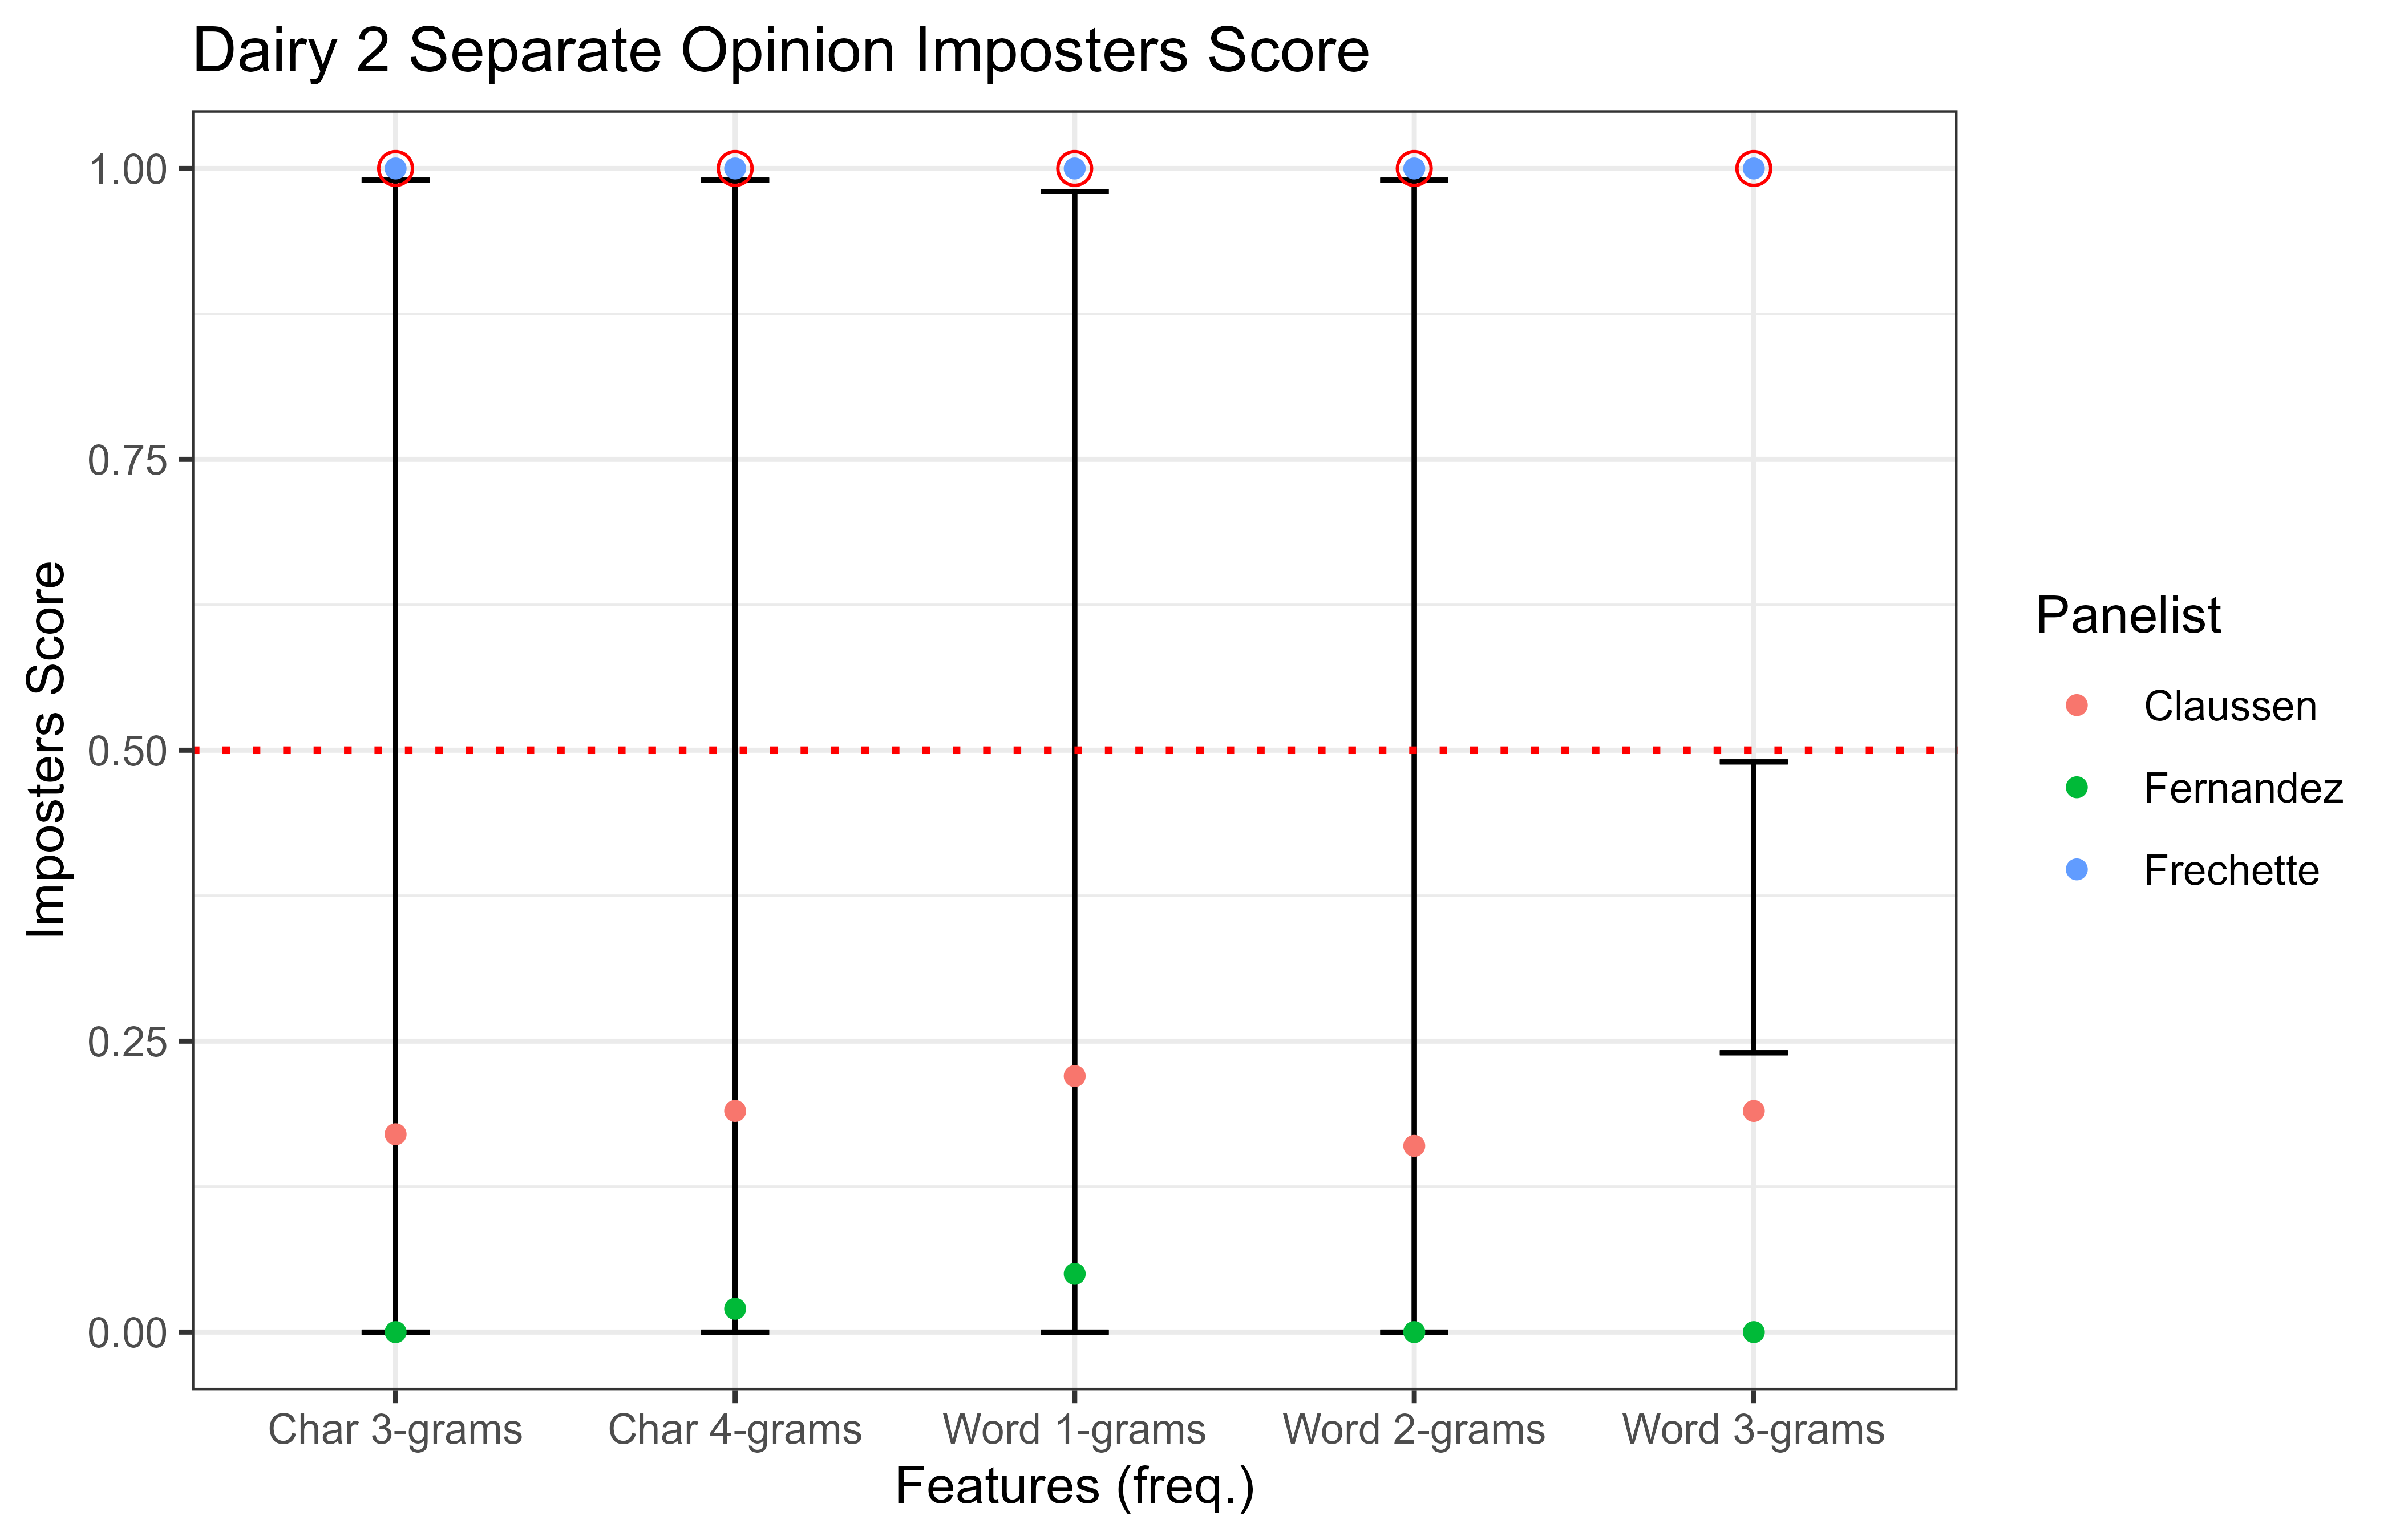
\includegraphics[width=0.85\textwidth,height=\textheight]{figures/imposters.png}

}

\caption{\label{fig-imposters}Authorship scores}

\end{figure}

Figure~\ref{fig-imposters} is a figure of authorship scores.

\hypertarget{analysis}{%
\section{Analysis}\label{analysis}}

The intuition of my proposal can be seen in Figure~\ref{fig-example}.
The original authors' measure of democracy changes abruptly at universal
suffrage, but my measures of Equal Access to Power and Civil Society to
Power changes more gradually. {[}\textbf{SK: See qmd code for an example
to insert figures, add a caption, and add a label that you can then
reference in text}{]}

\begin{figure}[tbp]

{\centering 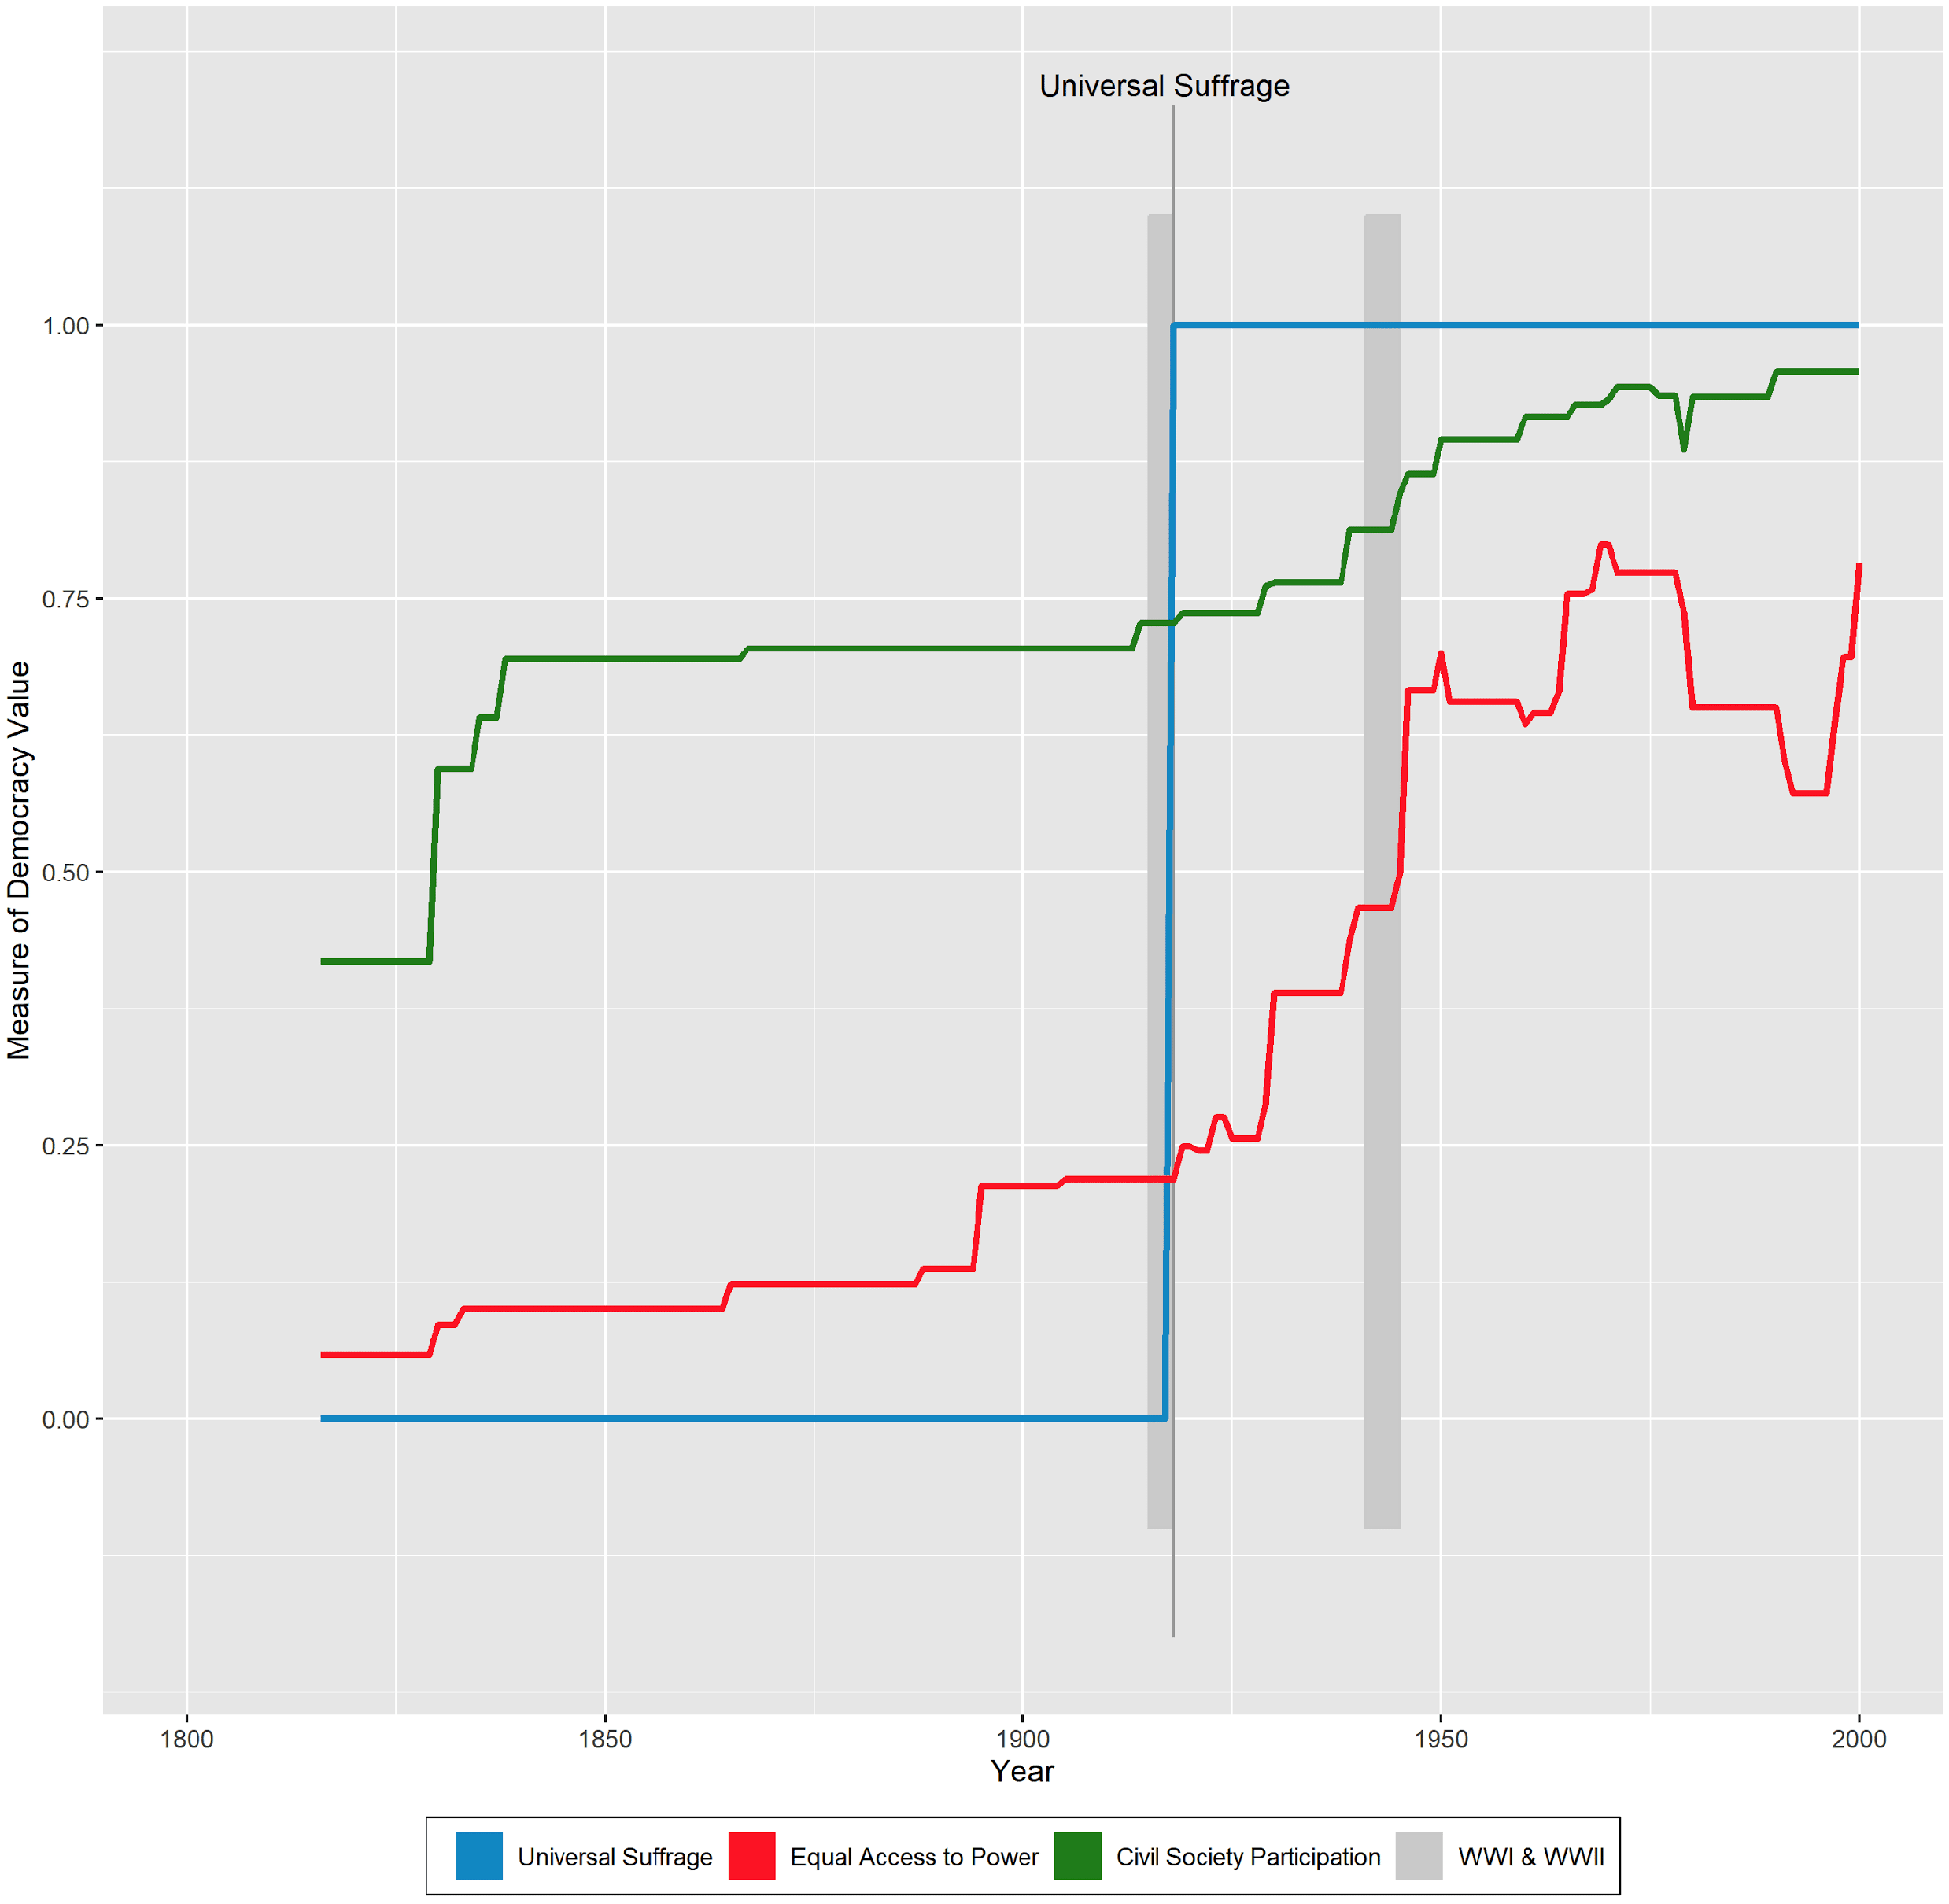
\includegraphics[width=0.5\textwidth,height=\textheight]{figures/image7.png}

}

\caption{\label{fig-example}Time Trends for Different Measures of
Democratic Participation in the United Kingdom, 1816-2000}

\end{figure}

Using data collected from V-Dem of the two new measures of
democratization, joint with the data used by \citep{scheve2012}, I
investigate the relationship between democracies that have given enough
political power to their lower socioeconomic classes and redistributive
taxation. I employ two main models. The first model uses a
differences-in-differences approach that estimates the causal effect of
democracy and wars of mass mobilization on inheritance taxation with an
ordinary least squares regression represented by:
\[T_{it} = \alpha + \beta_{1}D_{i,t - 1} + \beta_{2}W_{i,t - 1} + \gamma X_{i,t - 1} + \eta_{i} + \theta_{t} + \epsilon_{it},\]
where \(T_{it}\) is the top inheritance tax rate for direct descendants
for country \emph{i} in year \emph{t}.

\hypertarget{results}{%
\section{Results}\label{results}}

Table~\ref{tbl-main} shows the results of the regression. I find some
evidence for the importance of considering inequities in access to power
when investigating what causes increases in inheritance taxation. While
inconsistent, some models find that the effect of the lagged Equal
Access to Power index on top inheritance taxation is statistically
significant.

{[}\textbf{SK: The quarto code below puts in a figure into a markdown
table and calls it a table. Inserting tables are more complicated than
inserting figures, so a hack is to include the image of the table as I
have done here. Alternatively, you can also ask R to generate tables in
a .tex format and ask quarto read it in as a tex file. See Appendix.}{]}

\hypertarget{tbl-main}{}
\begin{longtable}[]{@{}l@{}}
\caption{\label{tbl-main}War Mobilization, Democracy, and Inheritance
Taxation, 1816-2000}\tabularnewline
\toprule\noalign{}
\endfirsthead
\endhead
\bottomrule\noalign{}
\endlastfoot
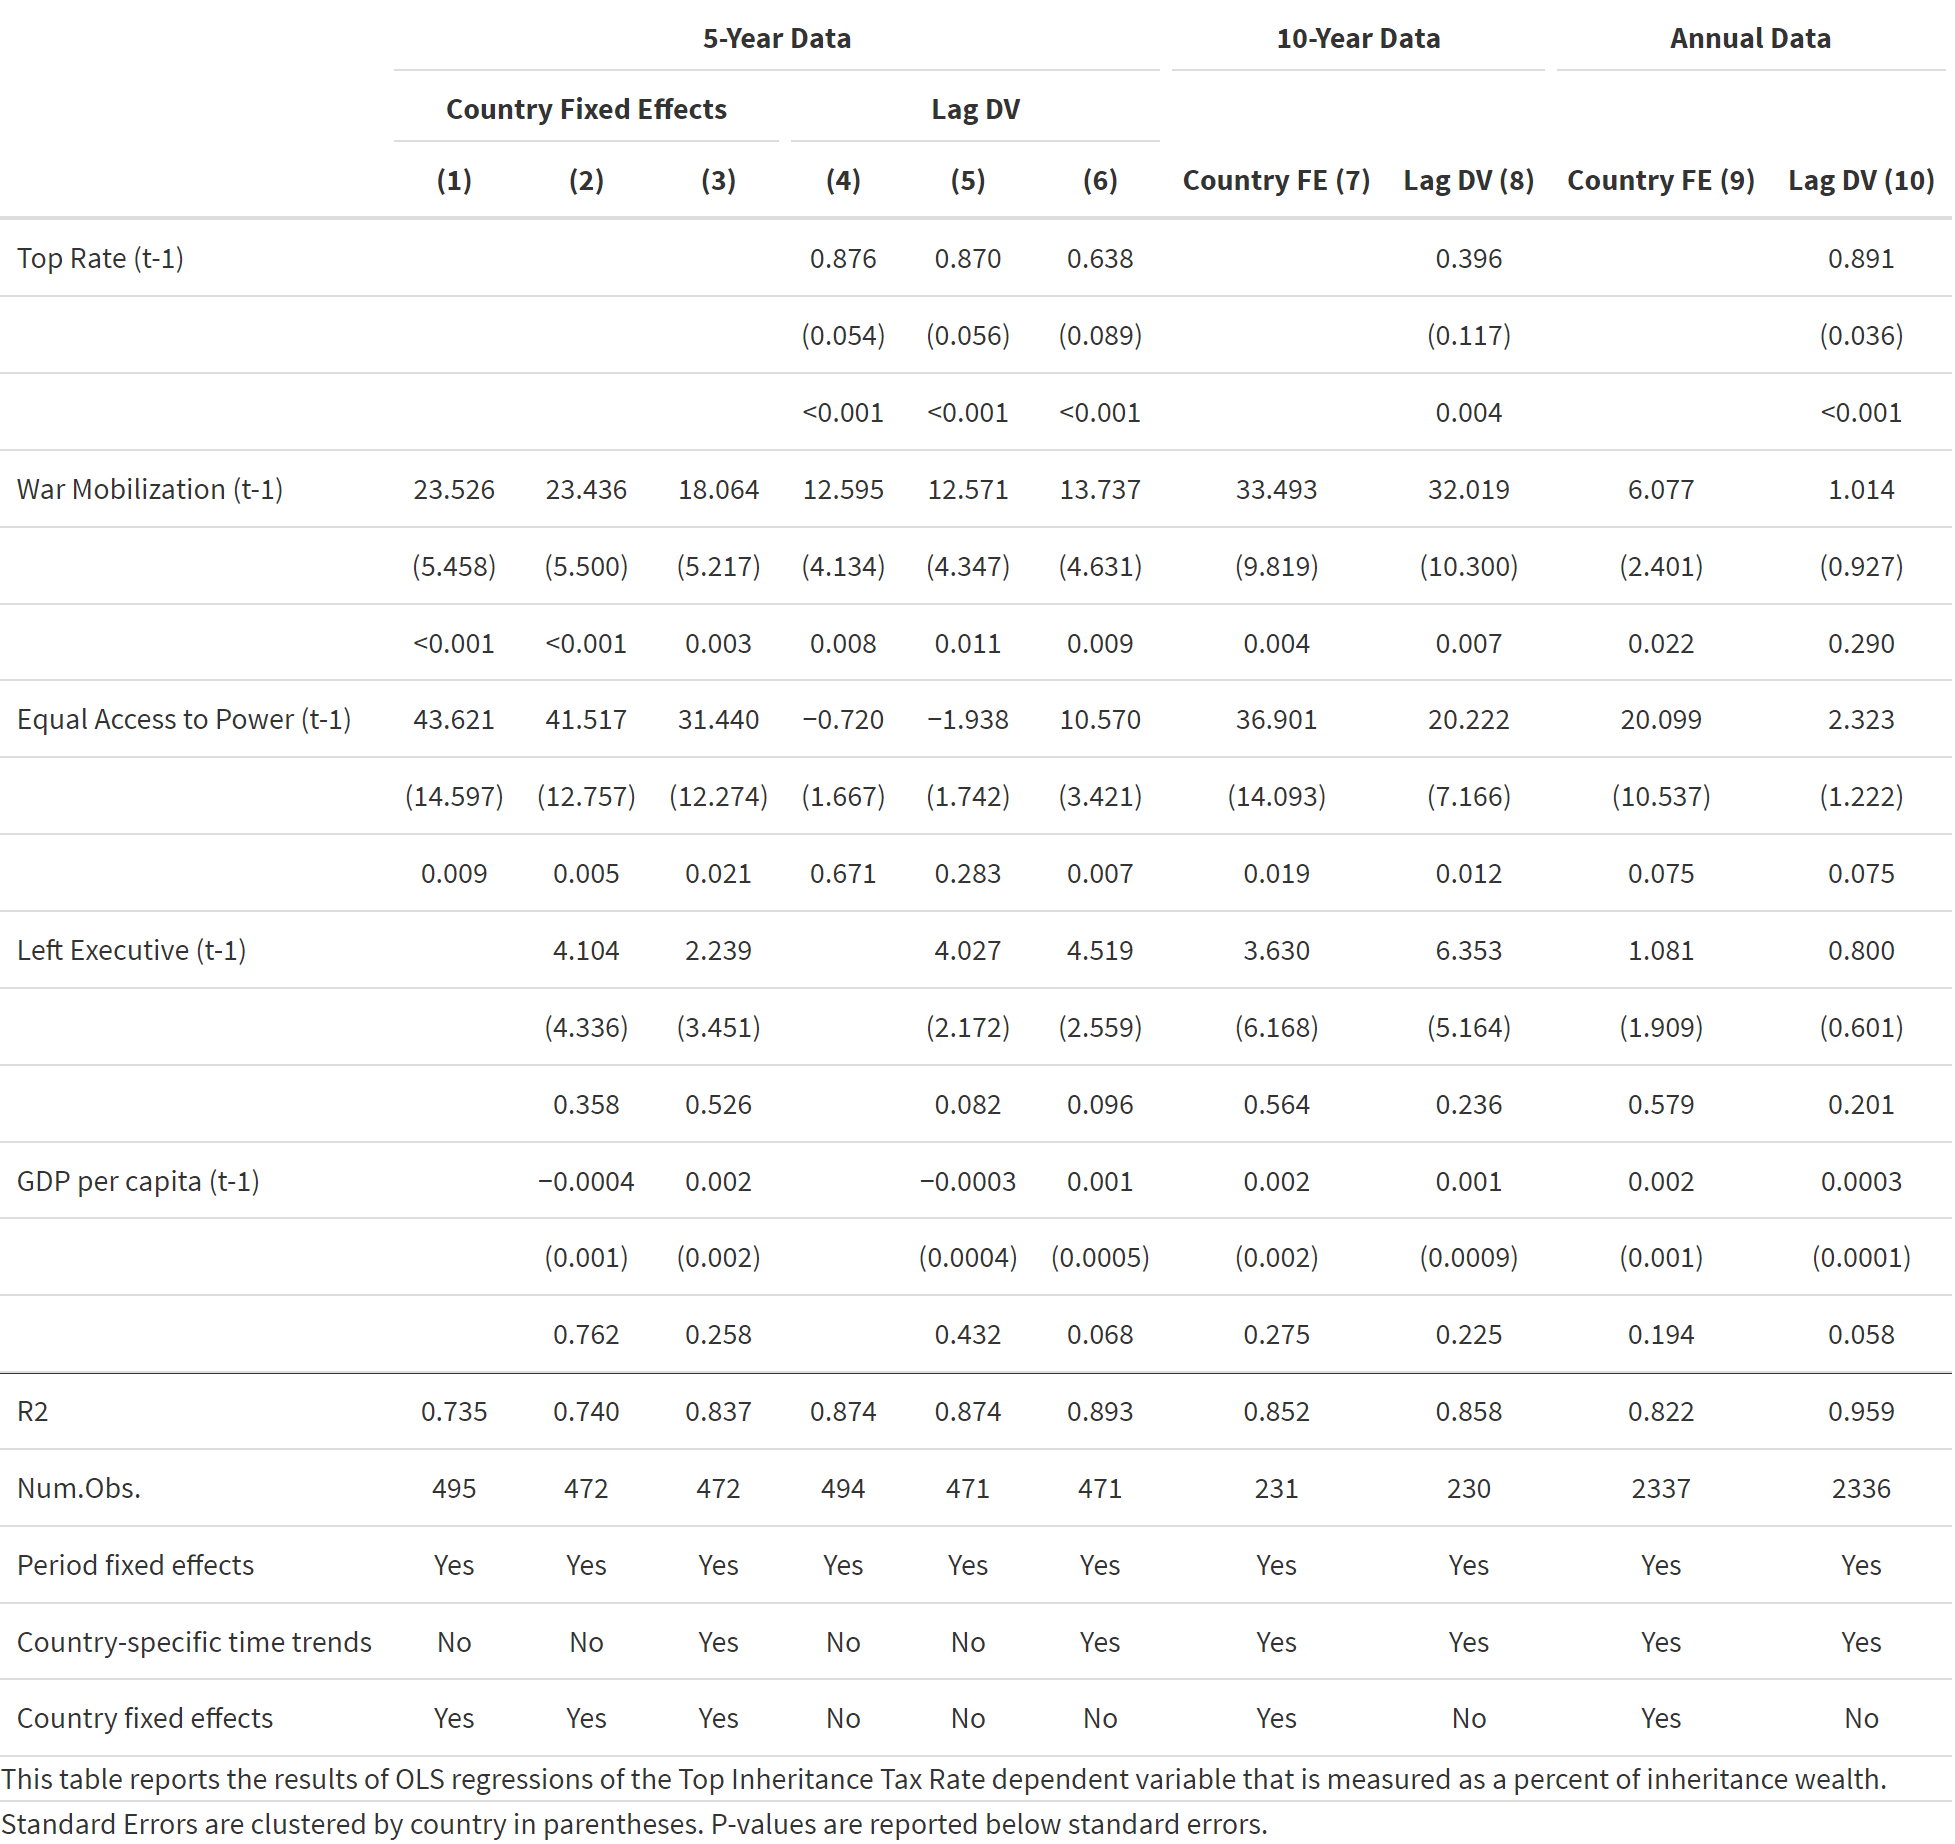
\includegraphics{figures/image3.png} \\
\end{longtable}

{[}\textbf{SK: Do not delete the two lines of quarto code that starts
with \texttt{:::\ \{\#refs\}}. This produces a list of references.}{]}

\hypertarget{refs}{}

\begin{CSLReferences}{0}{0}\end{CSLReferences}

\appendix

\hypertarget{appendix}{%
\section{Appendix}\label{appendix}}

\begin{table}
\caption{\textbf{tex version of modelsummary output}}

\begin{longtable}{lccc}
\toprule
  & (1) & (2) & (3) \\ 
\midrule\addlinespace[2.5pt]
War Mobilization (t - 1) & 23.017 & 21.464 & 18.468 \\ 
 & (6.086) & (5.737) & (5.556) \\ 
Universal Suffrage (t - 1) & 3.505 & 6.024 & 0.934 \\ 
 & (5.863) & (5.802) & (3.894) \\ 
Left Executive (t - 1) &  & 0.098 & 1.911 \\ 
 &  & (5.344) & (3.515) \\ 
GDP per Capita (t - 1) &  & 0.001 & 0.001 \\ 
 &  & (0.002) & (0.001) \\ 
Num.Obs. & 544 & 516 & 516 \\ 
Fixed Effects & Yes & Yes & Yes \\ 
Country-Specific Trends &  &  & Yes \\ 
Std.Errors & by: country & by: country & by: country \\ 
\bottomrule
\end{longtable}


\end{table}

Adding a \texttt{\{.appendix\}} next to your section header makes it an
Appendix.

Table \ref{tab:main-tex} is a table generated in LaTeX. LaTeX is a
different language than R or markdown. So, we denote that we are using
tex code explicitly by using the \texttt{\{=tex\}} tag. However, often
quarto can detect LaTeX code. For example, the notation
\texttt{\textbackslash{}ref\{tab:main-tex\}} used in the top of this
paragraph is tex code that quarto recognizes, and captures the number of
the table.

The file \texttt{tables/scheve-regression.tex} can be generated in your
R script. When you create the table with \texttt{modelsummary}, add
\texttt{output\ =\ "gt"} inside \texttt{modelsummary()}, and saving the
output of \texttt{modelsummary} into \texttt{gt::gtsave()}. For example,
this uses a simple example:

\begin{figure}[tbp]

{\centering 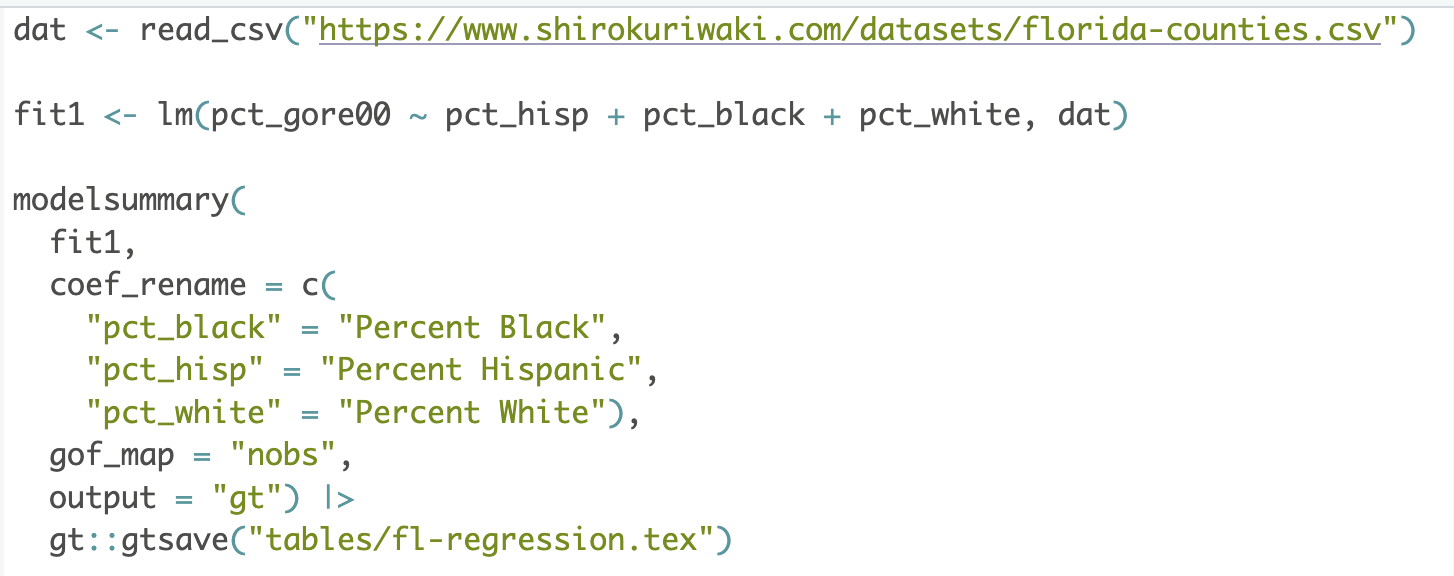
\includegraphics[width=0.8\textwidth,height=\textheight]{figures/codesnippet.png}

}

\end{figure}

Then, the code chunk starting with \texttt{\{=tex\}} in the quarto code
will read in the tex table, and add additional environments around it.
For more on these environments, see
\url{https://www.overleaf.com/learn/latex/Environments} and the chapters
in the website. ChatGPT should be quite good too at providing snippets
of LaTeX code. All the teaching fellows and instructors can help with
TeX.

% END BODY %%%%%%%%%%%%%%%%%%%%%%%%%%%%%%%%%%%%%%%%%%%%%%%%%%%%%%%%%%%%%%%%%%%%%



\end{document}
